\section{Experiments} \label{experiments}

\subsection{Experimental Setup}
\noindent \textbf{Model Architecture.} We implement \texttt{BiMol-Diff} using two distinct encoder-decoder Transformer models tailored for each task utilizing GeLU activations. Crucially, both tasks are trained for 200,000 steps using our proposed \textit{Token-aware noise schedule} (refer~\S\ref{adaptive noise}) over $T=2000$ diffusion steps. We adapt the architecture for each task as follows: for Molecule Generation (S2G), we employ a 6-encoder/12-decoder configuration ($d_{model}=1024$; $\approx 180$M parameters). The encoder processes
frozen SciBERT embeddings, while the decoder predicts the serialized
molecular graph sequence \(\tilde{G}\). This predicted graph sequence is
then deterministically mapped back into a canonical SMILES string for
evaluation. This variant is trained with a batch size of 64 and a learning rate of $5 \times 10^{-5}$. Conversely, for Molecule Captioning (G2S), we utilize a 6-encoder/9-decoder configuration ($d_{model}=512$; $\approx 63$M parameters) with a peak learning rate of $10^{-4}$. This model encodes serialized molecular structure using the AIS-based SMILES vocabulary augmented with learnable special tokens (\texttt{[HEAD]}, \texttt{[REL]}, \texttt{[TAIL]}, \texttt{[SEP]}), while the decoder generates captions utilizing the \texttt{bert-base-uncased} vocabulary~\cite{devlin-etal-2019-bert}.

\noindent \textbf{Datasets.} We evaluate our framework on two distinct datasets tailored to each task. For Molecule Generation (S2G), we utilize the ChEBI-20~\citep{edwards-etal-2022-translation} benchmark, comprising 33,010 molecules with SMILES strings restricted to a maximum length of 256. This dataset is partitioned into an 80\%/10\%/10\% split for training, validation, and testing, respectively. For Molecule Captioning (G2S), we employ a filtered subset of the M3-20M dataset~\cite{guo2025m320mlargescalemultimodalmolecule}, containing approximately 360,000 SMILES--description pairs. This subset, also divided into an 80\%/10\%/10\% split, pairs molecular graphs with diverse textual descriptions derived from curated scientific literature or synthesized via GPT-3.5.

\noindent \textbf{Baselines.} We compare \texttt{BiMol-Diff} against state-of-the-art (SoTA) autoregressive and diffusion-based methods for each task. 
For Molecule Generation (S2G), we benchmark against MolXPT~\citep{liu-etal-2023-molxpt} as a competitive autoregressive SMILES generator, and leading diffusion baselines including 3M-Diffusion~\citep{zhu20243mdiffusionlatentmultimodaldiffusion} and UTGDiff~\citep{xiang2025instructionbasedmoleculargraphgeneration}.
For Molecule Captioning (G2S), we compare against MolT5-Base~\citep{edwards-etal-2022-translation} as a standard SMILES$\rightarrow$text sequence-to-sequence baseline, GraphT5~\citep{kim2025grapht5unifiedmoleculargraphlanguage} as a recent graph--text model, and DiffuSeq~\citep{gong2023diffuseqsequencesequencetext} as a representative diffusion-based sequence generator.


\noindent \textbf{Evaluation Metrics.} For Molecule Captioning (G2S), we evaluate the quality of generated text using both surface-level and semantic measures. We report standard $n$-gram overlap metrics including BLEU \citep{papineni2002bleu}, METEOR \citep{banerjee2005meteor}, and ChrF++ \citep{popovic-2015-chrf}, alongside embedding-based metrics such as BERTScore-F1 \citep{zhang2020bertscoreevaluatingtextgeneration} and MAUVE \citep{pillutla2023mauvescoresgenerativemodels} to assess semantic alignment and distributional divergence. For Molecule Generation (S2G), we focus on structural fidelity and chemical plausibility. We report Exact Match accuracy to measure precise reconstruction of the ground-truth molecule. To assess the capture of chemical substructures, we compute structural overlap using Tanimoto similarity on MACCS, RDKit, and Morgan fingerprints. Finally, we report chemical validity to ensure the generated SMILES strings correspond to valid molecular graphs.

\subsection{Experimental Results}
\noindent \textbf{Molecule Captioning (G2S):} Table~\ref{molecule captioning} reports results on M3-20M. \texttt{BiMol-Diff} achieves the best overall performance on BLEU and ChrF++, reaching \textbf{0.567} BLEU and \textbf{0.734} ChrF++, which improves over the best performing autoregressive baseline (Text+Chem T5) by \textbf{4.6\%} and \textbf{4.7\%}, respectively. On semantic metrics, our model attains \textbf{0.843} BERTScore-F1 and \textbf{0.925} MAUVE, outperforming graph-aware baselines such as GraphT5, and consistently improving over diffusion models (e.g., DiffuSeq) across all reported metrics. While MolCA achieves the highest METEOR score, \texttt{BiMol-Diff} remains competitive (\textbf{0.626}) and offers a strong overall trade-off across surface and embedding-based measures, supporting the benefit of token-aware noising.


\noindent \textbf{Molecule Generation (S2G):} Table~\ref{molecule generation} summarizes results on ChEBI-20. \texttt{BiMol-Diff} attains an Exact Match of \textbf{0.262}, improving over both the best autoregressive adapter baseline (T5 Enc + MolXPT MLP) and the strongest diffusion baseline (UTGDiff), each at 0.227 (\textbf{+15.4\%} relative). This gain is reflected in fingerprint similarities, achieving \textbf{0.894} (MACCS), \textbf{0.791} (RDKit), and \textbf{0.762} (Morgan), including a \textbf{14.2\%} improvement in Morgan similarity over the best autoregressive baseline. Finally, \texttt{BiMol-Diff} maintains high chemical validity (\textbf{0.901}) while prioritizing reconstruction accuracy, whereas some baselines attain higher validity with weaker structural recovery.
% \vspace{-6mm}
\subsection{Ablation}
\begin{table*}[t!]
    \centering
    \small
    \setlength{\tabcolsep}{10pt}
    \resizebox{0.8\textwidth}{!}{%
    \begin{tabular}{l l c c c}
        \toprule
        \textbf{Noise Schedule} & \textbf{Mapping / Tokenizer} & \textbf{B} & \textbf{CrF++} & \textbf{M} \\
        \midrule
        
        % --- Partition 1: Noise Strategy Ablation ---
        \multicolumn{5}{l}{\textbf{\textit{Impact of Noise Schedule \& Mapping Function}}} \\
        Uniform & Sqrt Schedule & 0.495 & 0.682 & 0.531 \\
        Token-Aware & Cosine Mapping & 0.548 & 0.720 & 0.595 \\
       
        \rowcolor{yellow!25}
        Token-Aware (Ours) & Linear Mapping & \textbf{0.567} & \textbf{0.734} & \textbf{0.626} \\
        
        \midrule
        
        % --- Partition 2: Tokenization Ablation ---
        \multicolumn{5}{l}{\textbf{\textit{Impact of Molecular Tokenization}}} \\
        % Note: These rows assume the noise/mapping is fixed to the best setting (Token-Aware + Linear)
        Token-Aware (Linear) & Regex-based & 0.558 & 0.714 & 0.606 \\
        Token-Aware (Linear) & Atom-level & 0.563 & 0.722 & 0.613 \\
        % Highlight the best tokenization (AIS)
        \rowcolor{yellow!25}
        Token-Aware (Linear) & Atoms-in-SMILES (AIS) & \textbf{0.567} & \textbf{0.734} & \textbf{0.626} \\
        \bottomrule
    \end{tabular}}
    \caption{Ablation study on the M3-20M dataset. We analyze the impact of different (\textbf{Top}) Noise Schedules \& Mapping Functions and (\textbf{Bottom}) Tokenization strategies on molecule captioning performance. \texttt{BiMol-Diff} (Token-Aware + Linear) with Atoms-in-SMILES (AIS) tokenization yields the best results.}
    \label{tab:ablation_study}
    \vspace{-4mm}
\end{table*}

\noindent We analyze three aspects of \texttt{BiMol-Diff}: (i) the proposed token-aware noising strategy and its mapping function, (ii) the effect of molecular tokenization, and (iii) decoding efficiency of \texttt{BiMol-Diff}.

\noindent \textbf{(i) Impact of noise schedule and choice of mapping function.}
Table~\ref{tab:ablation_study} (top) shows that replacing a uniform corruption schedule (\textit{sqrt}) with our token-aware schedule yields a substantial improvement (0.495$\rightarrow$0.567 BLEU; 0.682$\rightarrow$0.734 ChrF++; 0.531$\rightarrow$0.626 METEOR). Among mapping choices, the linear mapping performs best, indicating that explicitly allocating lower corruption to harder-to-recover tokens is beneficial for caption recovery. Figure~\ref{noise schedule} visualizes how token-aware schedules differ from a global \textit{sqrt} schedule. Instead of applying the same noise profile to all positions, we learn per-token schedules that modulate the corruption level according to token difficulty: positions with higher denoising loss receive more conservative corruption (lower noise at intermediate timesteps), while easier positions can be noised more aggressively. This selective corruption better preserves content during the forward process and improves recoverability in the reverse process, which aligns with the gains observed in the main results (Table~\ref{molecule captioning},~\ref{molecule generation}).
\begin{figure}[ht!]
    \centering
    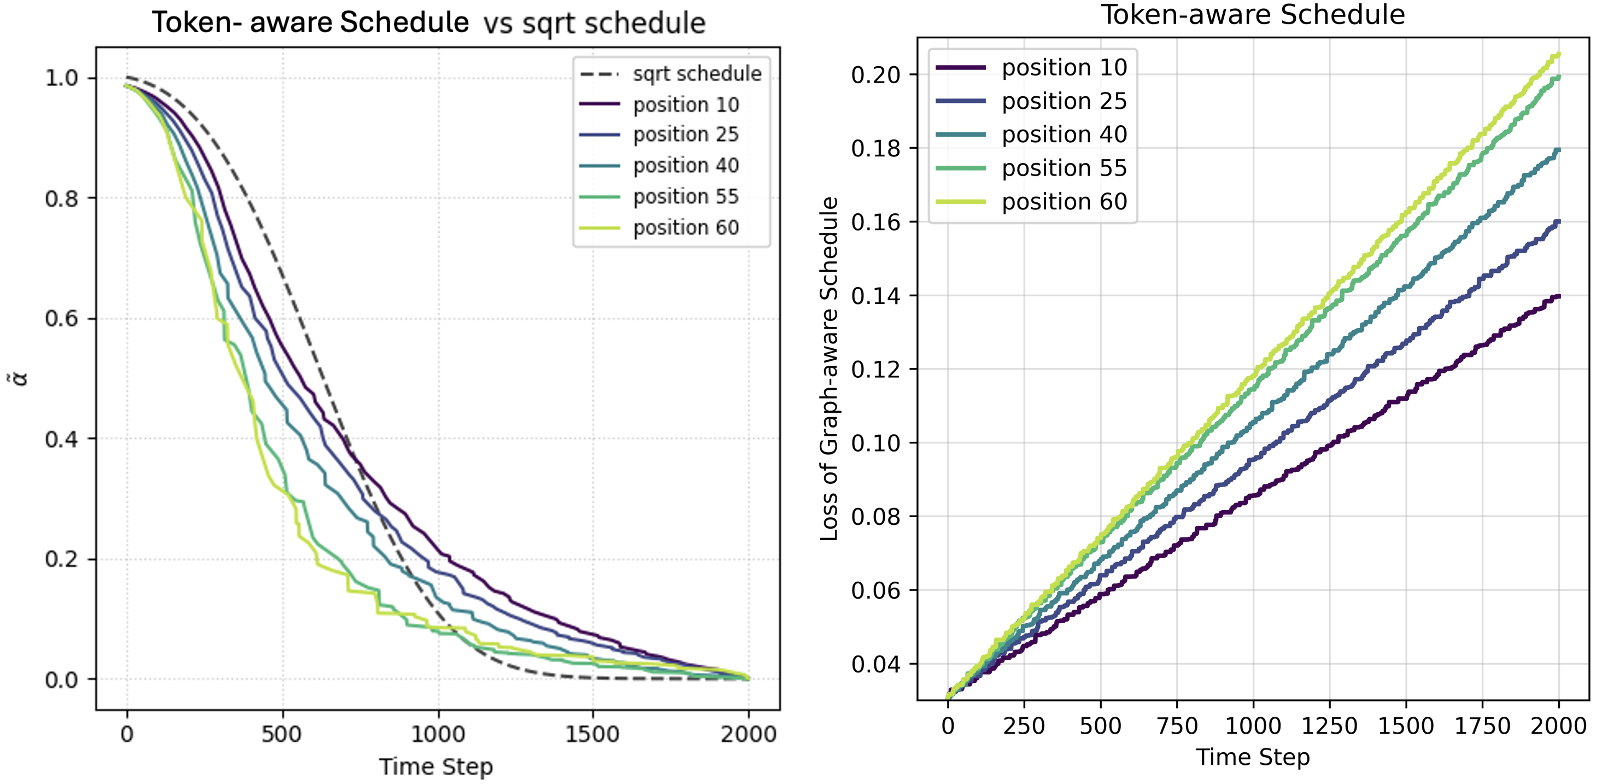
\includegraphics[width=\linewidth]{latex/Images/BiMolDiff.png}
    \caption{Token-aware noising vs.\ uniform sqrt schedule (captioning). \emph{Left:} the learned token-wise schedules apply non-uniform corruption across positions compared to a global sqrt schedule. \emph{Right:} token-wise difficulty profiles are used to construct schedules that apply more conservative corruption to harder-to-recover tokens.}
    \label{noise schedule}
\end{figure}
\vspace{-3mm}\\
\noindent \textbf{(ii) Impact of molecular tokenization.}
Table~\ref{tab:ablation_study} (bottom) applies the best noising configuration (token-aware + linear) with different molecular tokenizers. Our current framework uses an AIS-based SMILES tokenizer for a stable, deterministic segmentation that preserves SMILES syntax (e.g., bracketed atoms and ring/branch symbols) and enables straightforward serialization, the tokenizer is plug-and-play and can be swapped without changing the denoising objective or architecture. We observe a clear monotonic trend: regex-based SMILES tokenization underperforms atom-level tokens, while Atoms-in-SMILES (AIS) yields the strongest performance across all reported metrics.

% \noindent \textbf{(iii) Decoding Efficiency.} As diffusion models inherently require iterative refinement, we analyze the quality-latency trade-off. We observe that reducing the number of reverse steps yields substantial speedups at the cost of generation fidelity. To prioritize modeling performance over speed in our main analysis, we utilize $T{=}2000$ for all reported experiments, deferring efficiency optimizations to future work.

% \noindent Table \ref{tab:efficiency_g2s_merged} analyzes the trade-off between inference speed and generation quality for Graph-to-Sequence tasks. First, comparing within the diffusion family, \texttt{BiMol-Diff} demonstrates significantly better efficiency than the standard DiffuSeq baseline. At 2000 steps, our model achieves a BLEU score of 0.567 while requiring only 89 seconds to process a batch, representing a 3.6$\times$ speedup over DiffuSeq (317 seconds) with better output generation.

%%%%%%%%
\noindent \textbf{(iii) Decoding Efficiency.} Given the iterative nature of diffusion models, we examine the trade-off between generation quality and inference latency. Reducing the number of reverse steps leads to substantial speedups, albeit with a degradation in output fidelity. To focus on modeling performance, all primary results are reported with $T{=}2000$ steps. Table~\ref{tab:efficiency_g2s_merged} presents the quality-latency trade-off for Graph-to-Sequence tasks. Within the diffusion family, \texttt{BiMol-Diff} exhibits markedly improved efficiency over DiffuSeq. At $T{=}2000$, it achieves a BLEU score of 0.567 in 89 seconds per batch, yielding a $3.6\times$ speedup over DiffuSeq (317 seconds), while also improving generation quality.
\begin{table}[ht!]
\centering
\small
\setlength{\tabcolsep}{4pt}
\renewcommand{\arraystretch}{1.2}

\resizebox{\columnwidth}{!}{%
\begin{tabular}{l c c c c c}
\toprule
\textbf{Method} &
\textbf{Params} &
\textbf{Steps} &
\textbf{Time (s)} &
\textbf{Speedup} &
\textbf{BLEU $\uparrow$} \\
\midrule
\multicolumn{6}{l}{\textit{\textbf{Autoregressive Baselines}}} \\
MolT5-Base \citep{edwards-etal-2022-translation} & 220M & -- & $<$5s & -- & 0.452 \\
Text+Chem T5 \citep{christofidellis2023textchemt5} & 223M  & -- & $<$5s & -- & 0.542 \\
\midrule
\multicolumn{6}{l}{\textit{\textbf{Diffusion Baselines}}} \\
DiffuSeq \citep{gong2023diffuseqsequencesequencetext}     & 91M  & 2000 & 317s & $1.0\times$ (Ref) & 0.532 \\
\midrule
\multicolumn{6}{l}{\textit{\textbf{Ours}}} \\
\textbf{BiMol-Diff} & 63M & 2000 & 89s & $3.6\times$ & \textbf{0.567} \\
\textbf{BiMol-Diff} & 63M & 1000 & 45s & $7.0\times$ & 0.551 \\
\textbf{BiMol-Diff} & 63M & 500  & 23s & $13.8\times$ & 0.365 \\
\textbf{BiMol-Diff} & 63M & 100  & 5s  & $63.4\times$ & 0.312 \\
\bottomrule
\end{tabular}%
}
\caption{Inference efficiency comparison on the G2S task. We compare \texttt{BiMol-Diff} against the best Autoregressive (AR) and Diffusion baselines from Table \ref{molecule captioning}. Time is measured as total inference time for a batch size of 50 on a single NVIDIA V100 GPU.}
\label{tab:efficiency_g2s_merged}

\end{table}
\noindent When compared to Autoregressive (AR) baselines, our model shows a clear operational boundary. In the high-quality output range (1000--2000 steps), \texttt{BiMol-Diff} outperforms the strongest AR baseline, Text+Chem T5 (0.542 BLEU), confirming that the extra computational time yields better text generation. However, the model struggles when pushed for extreme speed. As we reduce the inference steps below 1000, we observe a sharp drop in performance. At 500 steps, although the inference time improves to 23 seconds (13.8$\times$ speedup), the BLEU score falls to 0.365, which is lower than even the base MolT5 model (0.452). This indicates that \texttt{BiMol-Diff} requires a minimum threshold of denoising steps (approximately 1000) to maintain its advantage. Our model is ideal for high-precision generation and simple AR models remain the better choice for low-latency applications.